\documentclass{article}
\usepackage{amsmath}
\usepackage{amssymb}
\usepackage{graphicx}
\usepackage{float}
\usepackage[margin=1cm,footskip=0.25cm]{geometry}
\usepackage{tikz}

\begin{document}
\begin{center}
    \textbf{\LARGE Theoretische Informatik}
\end{center}

\section*{Alphabete, Wörter und Sprachen}
\begin{minipage}[t]{0.45\textwidth}
    \subsection*{Alphabete}
    Ein \textbf{Alphabet} $\Sigma$ ist eine endliche, nichtleere Menge von Symbolen.
    
    \subsection*{Sprachen}
    Eine \textbf{Sprache} $L$ über einem Alphabet $\Sigma$ ist eine Menge von Wörtern, die aus Symbolen von $\Sigma$ bestehen. Eine Sprache kann endlich oder unendlich sein. Die leere Sprache wird mit $\emptyset$ bezeichnet.
\end{minipage}
\hfill
\begin{minipage}[t]{0.45\textwidth}
    \subsection*{Wörter}
    Ein \textbf{Wort} $w$ ist eine endliche Folge von Symbolen aus einem Alphabet $\Sigma$. Die Länge eines Wortes $w$ wird mit $|w|$ bezeichnet. Das leere Wort wird mit $\varepsilon$ dargestellt und hat die Länge 0.
    Die Menge aller Wörter über einem Alphabet $\Sigma$ wird mit $\Sigma^*$ bezeichnet (Kleenesche Hülle). 
\end{minipage}
\section*{Endliche Automaten}
\begin{minipage}[t]{0.45\textwidth}
    \subsection*{Deterministische endliche Automaten (DEA)}
    Ein DEA ist ein 5-Tupel $M = (Q, \Sigma, \delta, q_0, F)$, wobei:
    \begin{itemize}
        \item $Q$ eine endliche Menge von Zuständen ist,
        \item $\Sigma$ ein Alphabet ist,
        \item $\delta: Q \times \Sigma \to Q$ die Übergangsfunktion ist,
        \item $q_0 \in Q$ der Startzustand ist,
        \item $F \subseteq Q$ die Menge der Endzustände ist.
    \end{itemize}
    \textbf{Übergangsfunktion:} $\delta(q_0, a_1) = q_1$

    Ein Wort $w \in \Sigma^*$ wird akzeptiert, wenn es von $M$ verarbeitet wird und der Endzustand in $F$ liegt.
\end{minipage}
\hfill
\begin{minipage}[t]{0.45\textwidth}
    \subsection*{Nichtdeterministische endliche Automaten (NEA)}
    Ein NEA ist ähnlich aufgebaut, aber die  Übergangsfunktion $\delta$ kann mehrere Zustände für ein Symbol zurückgeben: 
    $\delta: Q \times \Sigma \to 2^Q$. Ein NEA akzeptiert ein Wort, wenn es mindestens einen Pfad gibt, der das Wort vollständig verarbeitet und in einem Endzustand endet.

    \begin{center}
        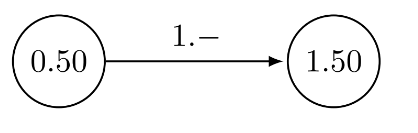
\includegraphics[scale=0.5]{images/ea.png}
    \end{center}
\end{minipage}

\vspace{0.5cm}

\section*{Kontextfreie Grammatiken}
\begin{minipage}[t]{0.45\textwidth}
    \subsection*{Definition}
    Eine \textbf{kontextfreie Grammatik} (KFG) ist ein 4-Tupel $G = (V, \Sigma, P, S)$, wobei:
    \begin{itemize}
        \item $V$ eine endliche Menge von Variablen ist,
        \item $\Sigma$ ein Alphabet ist (Terminale),
        \item $P$ eine endliche Menge von Produktionen ist,
        \item $S \in V$ das Startsymbol ist.
    \end{itemize}
    \subsection*{Produktionen}
    Eine Produktion hat die Form $A \to \alpha$, wobei $A \in V$ und $\alpha \in (V \cup \Sigma)^*$. Die Ableitung eines Wortes erfolgt durch wiederholtes Anwenden der Produktionen.
\end{minipage}
\hfill
\begin{minipage}[t]{0.45\textwidth}
    \subsection*{Ableitung}
    Ein Wort $w$ wird aus $G$ abgeleitet, wenn es durch eine endliche Folge von Produktionen aus dem Startsymbol $S$ entsteht. Die Menge aller Wörter, die aus $G$ abgeleitet werden können, bildet die Sprache $L(G)$ der Grammatik.
    \begin{center}
        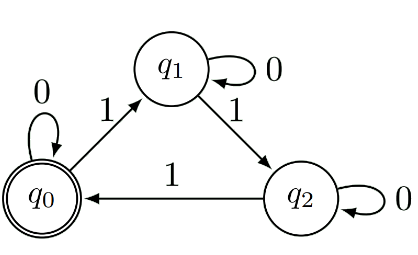
\includegraphics[scale=0.5]{images/kfg.png}
    \end{center}
\end{minipage}
\section*{Kellerautomaten (KA)}
\begin{minipage}[t]{0.45\textwidth}
    Ein \textbf{Kellerautomat} (Pushdown automata) (PDA) ist ein endlicher Automat, der zusätzlich einen Keller (Stack) hat. 
    Er kann Symbole auf den Stack legen und entfernen. Ein Kellerautomat wird durch ein 7-Tupel $M = (Q, \Sigma, \Gamma, \delta, q_0, Z_0, F)$ definiert:
    \begin{itemize}
        \item $Q$ eine endliche Menge von Zuständen,
        \item $\Sigma$ ein Eingabealphabet,
        \item $\Gamma$ ein Kelleralphabet,
        \item $\delta: Q \times \Sigma \times \Gamma \to 2^{Q \times \Gamma^*}$ die Übergangsfunktion,
        \item $q_0 \in Q$ der Startzustand,
        \item $Z_0 \in \Gamma$ das Startsymbol des Kellers,
        \item $F \subseteq Q$ die Menge der Endzustände.
    \end{itemize}
    \textbf{Übergangsfunktion:} $\delta(q_0, a_1, Z_0) = (q_1, Z_0 a_2)$
    \begin{enumerate}
        \item Ist im Zustand $q_0$ 
        \item wird das Symbol $a_1$ gelesen,
        \item wird das Symbol $Z_0$ vom Keller gepopt,
        \item wechselt der Automat in den Zustand $q_1$,
        \item und legt das Symbol $Z_0 a_2$ auf den Keller.
    \end{enumerate}
    
    Ein Kellerautomat akzeptiert ein Wort, wenn es in einem Endzustand endet und der Keller leer ist.
\end{minipage}
\hfill
\begin{minipage}[t]{0.45\textwidth}
    \begin{center}
    \usetikzlibrary{automata, positioning}
    \begin{tikzpicture}[shorten >=1pt, node distance=3cm, on grid, auto]
        % States
        \node[state, initial] (q0) {$q_0$};
        \node[state, right=of q0] (q1) {$q_1$};

        % q0 loop
        \path[->]
            % (q0) edge[loop above] node[align=left] {$a, Z_0/A Z_0$\\$a, A/AA$} ()
            (q0) edge[left] node[above] {$b, A/\varepsilon$} (q1);
    \end{tikzpicture}
    \end{center}
    \textit{Legende: $x, y/z$ bedeutet: lese $x$, poppe $y$ vom Keller, pushe $z$ auf den Keller.}
\end{minipage}
\end{document}